\pagenumbering{arabic}
\section{AES加解密算法}
\begin{figure}[thbp!]
	\centering
	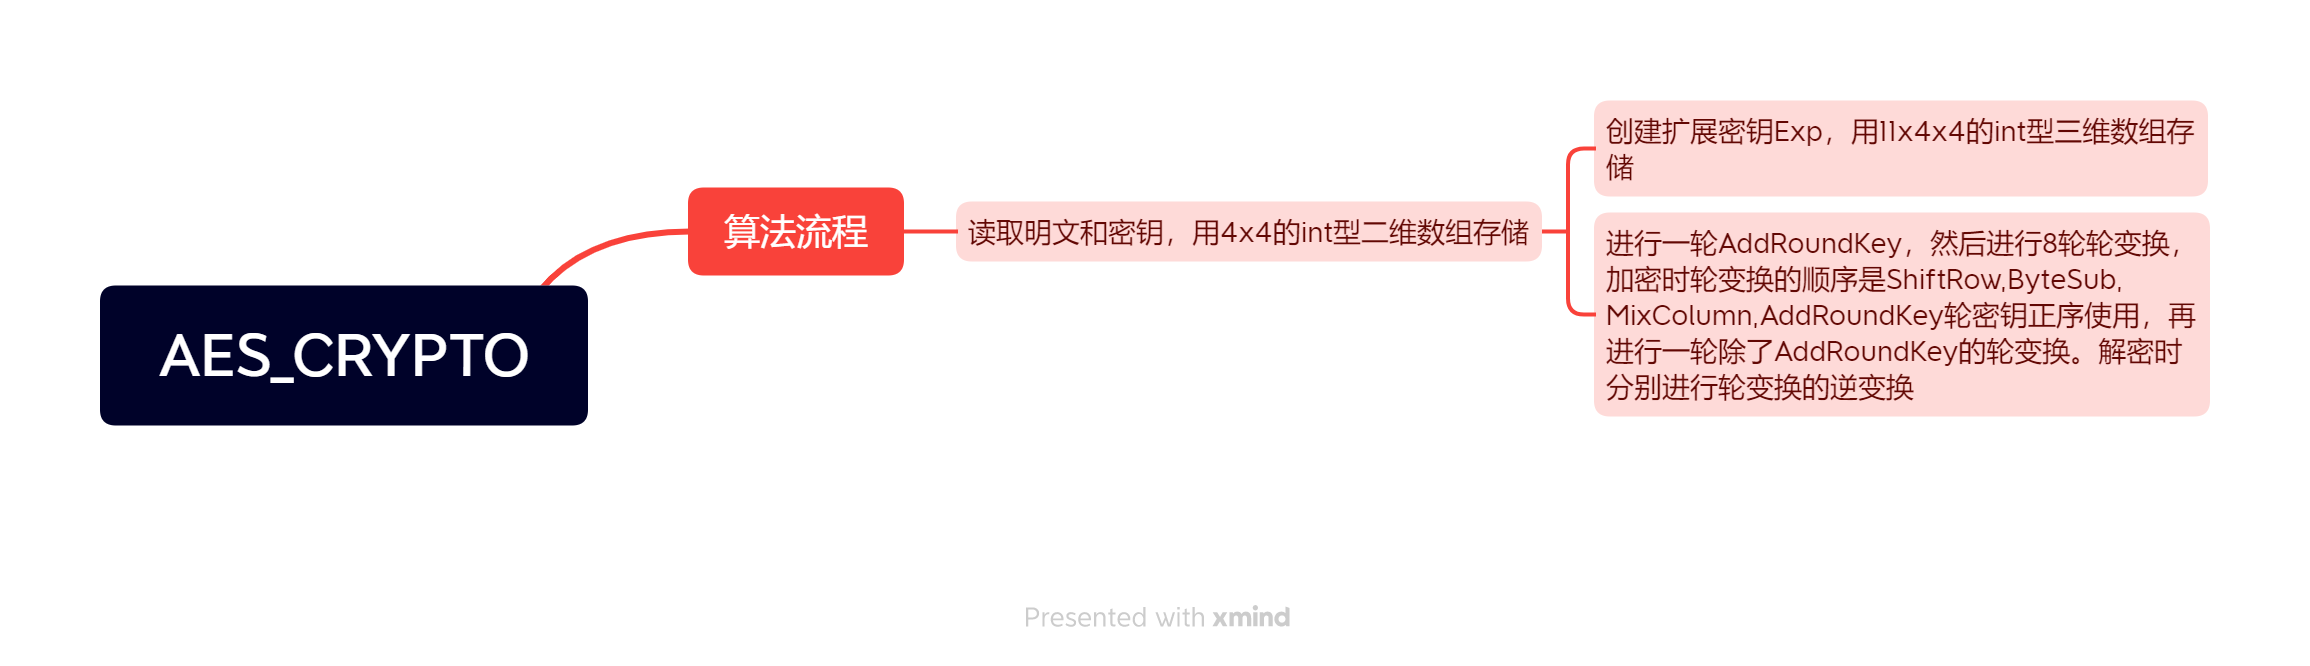
\includegraphics[height=6 CM,width=18cm]{figure/001.png}
	\caption{AES算法流程图}
	\label{fig:AES算法流程图}
\end{figure}
\begin{figure}[thbp!]
	\centering
	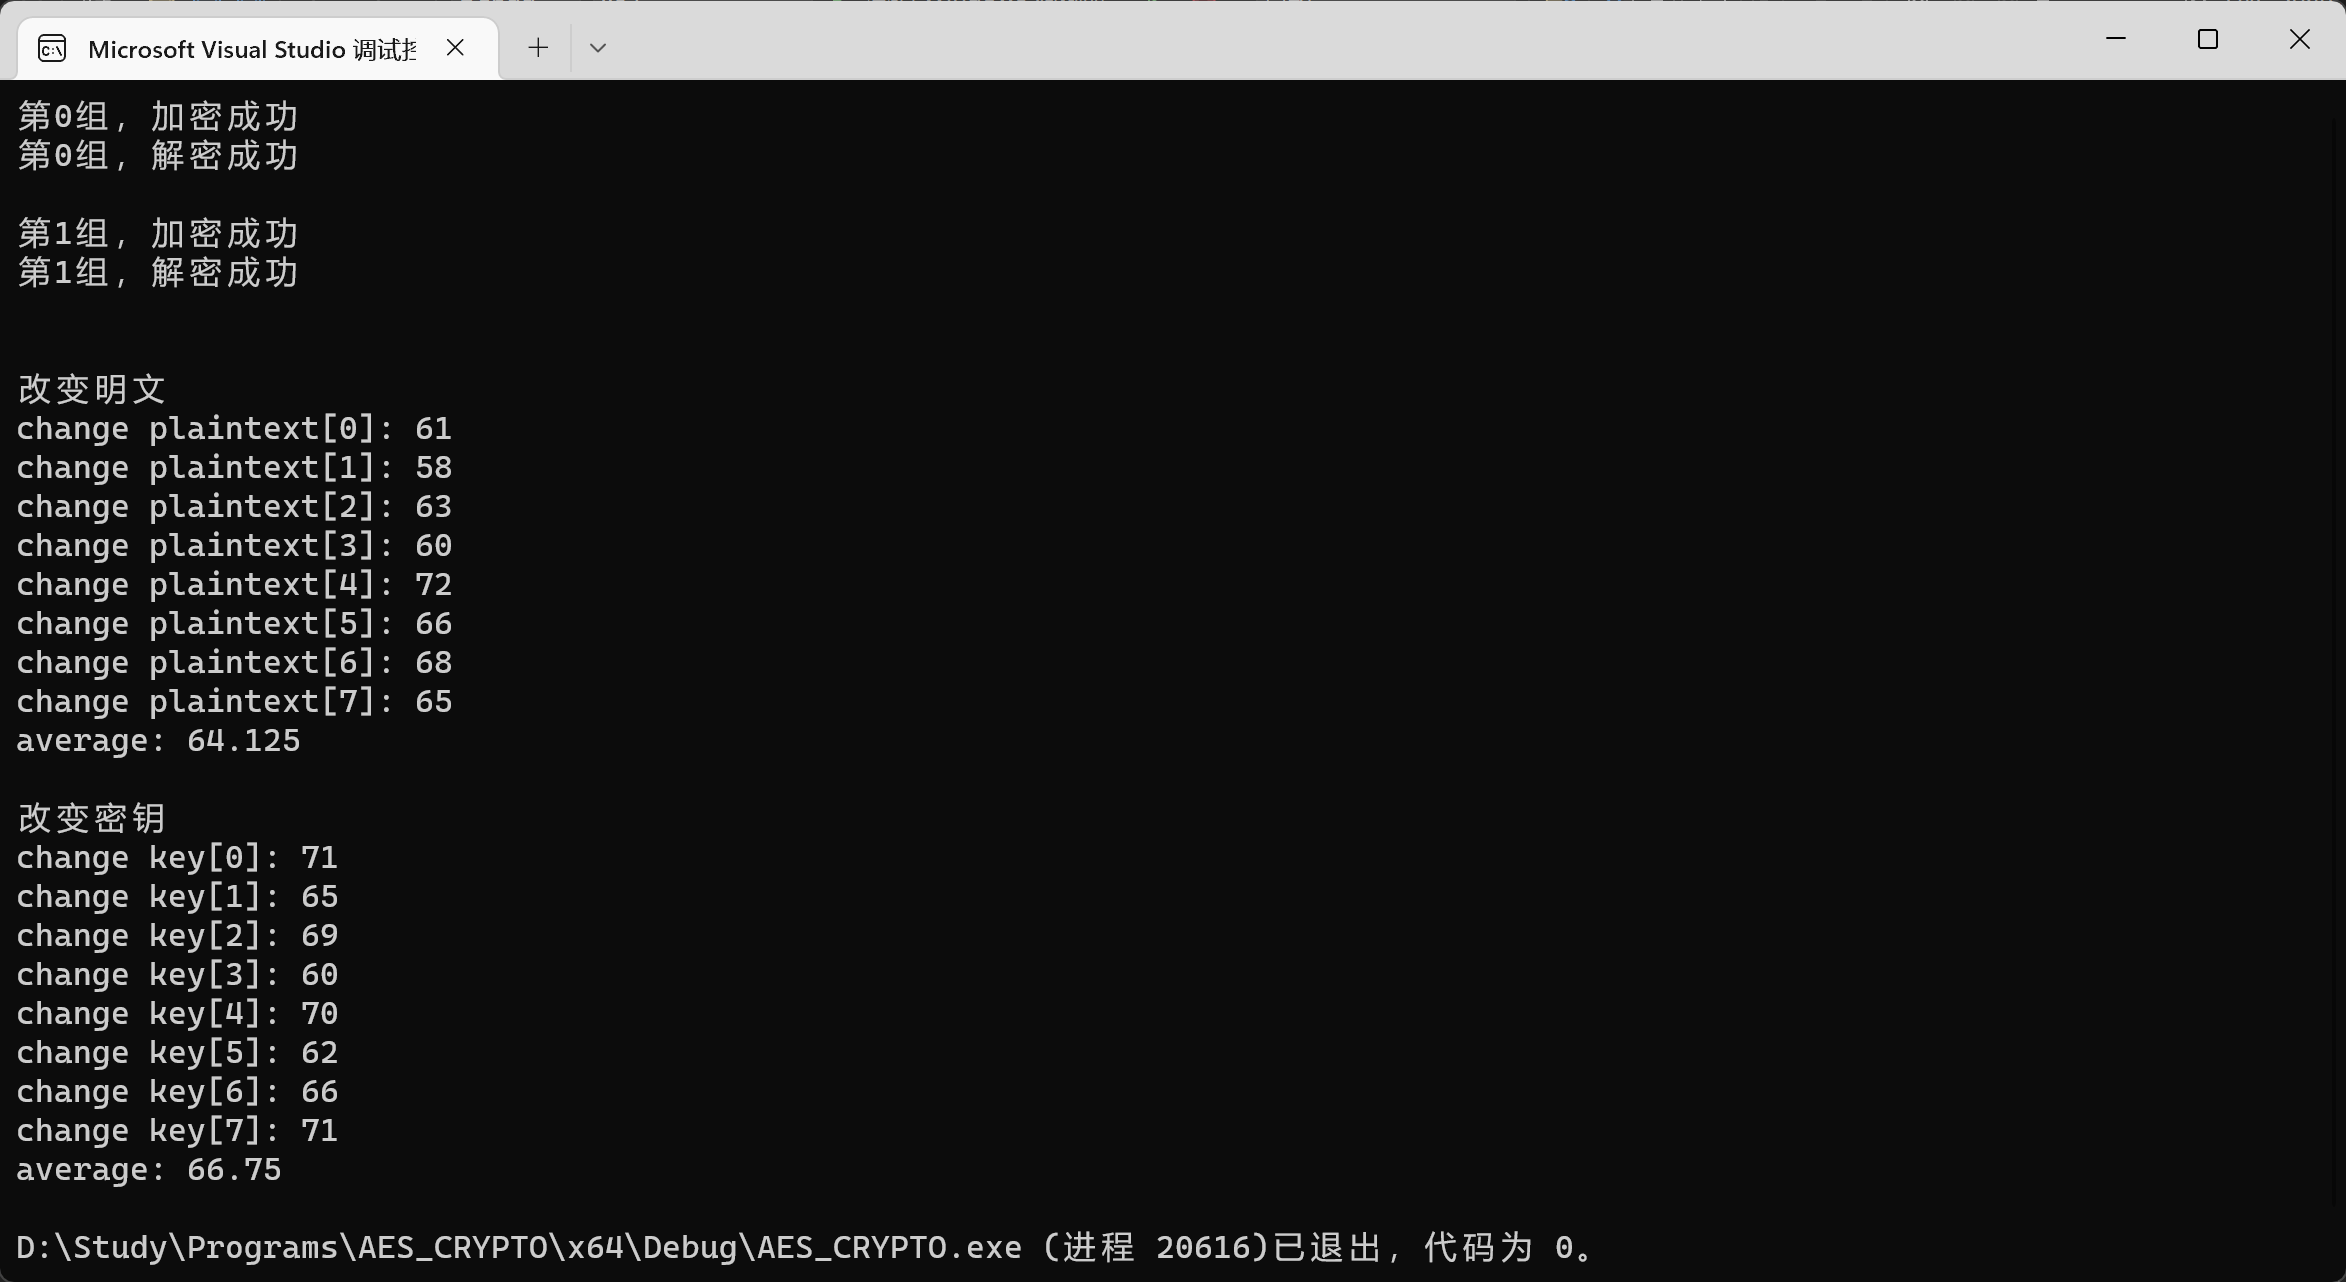
\includegraphics[height=10 CM]{figure/002}
	\caption{输出结果演示}
	\label{fig:输出结果演示}
\end{figure}
Nb=Nk=4,Nr=10\\
2组样例加解密全部正确,改变plaintext1位,8次得到的雪崩效应平均值是64.125,改变key1位,8次计算得到的雪崩效应平均值是66.75\\

接下来概括性写一下中间生成结果(以第0组数据为例)\\
\begin{figure}[thbp!]
	\centering
	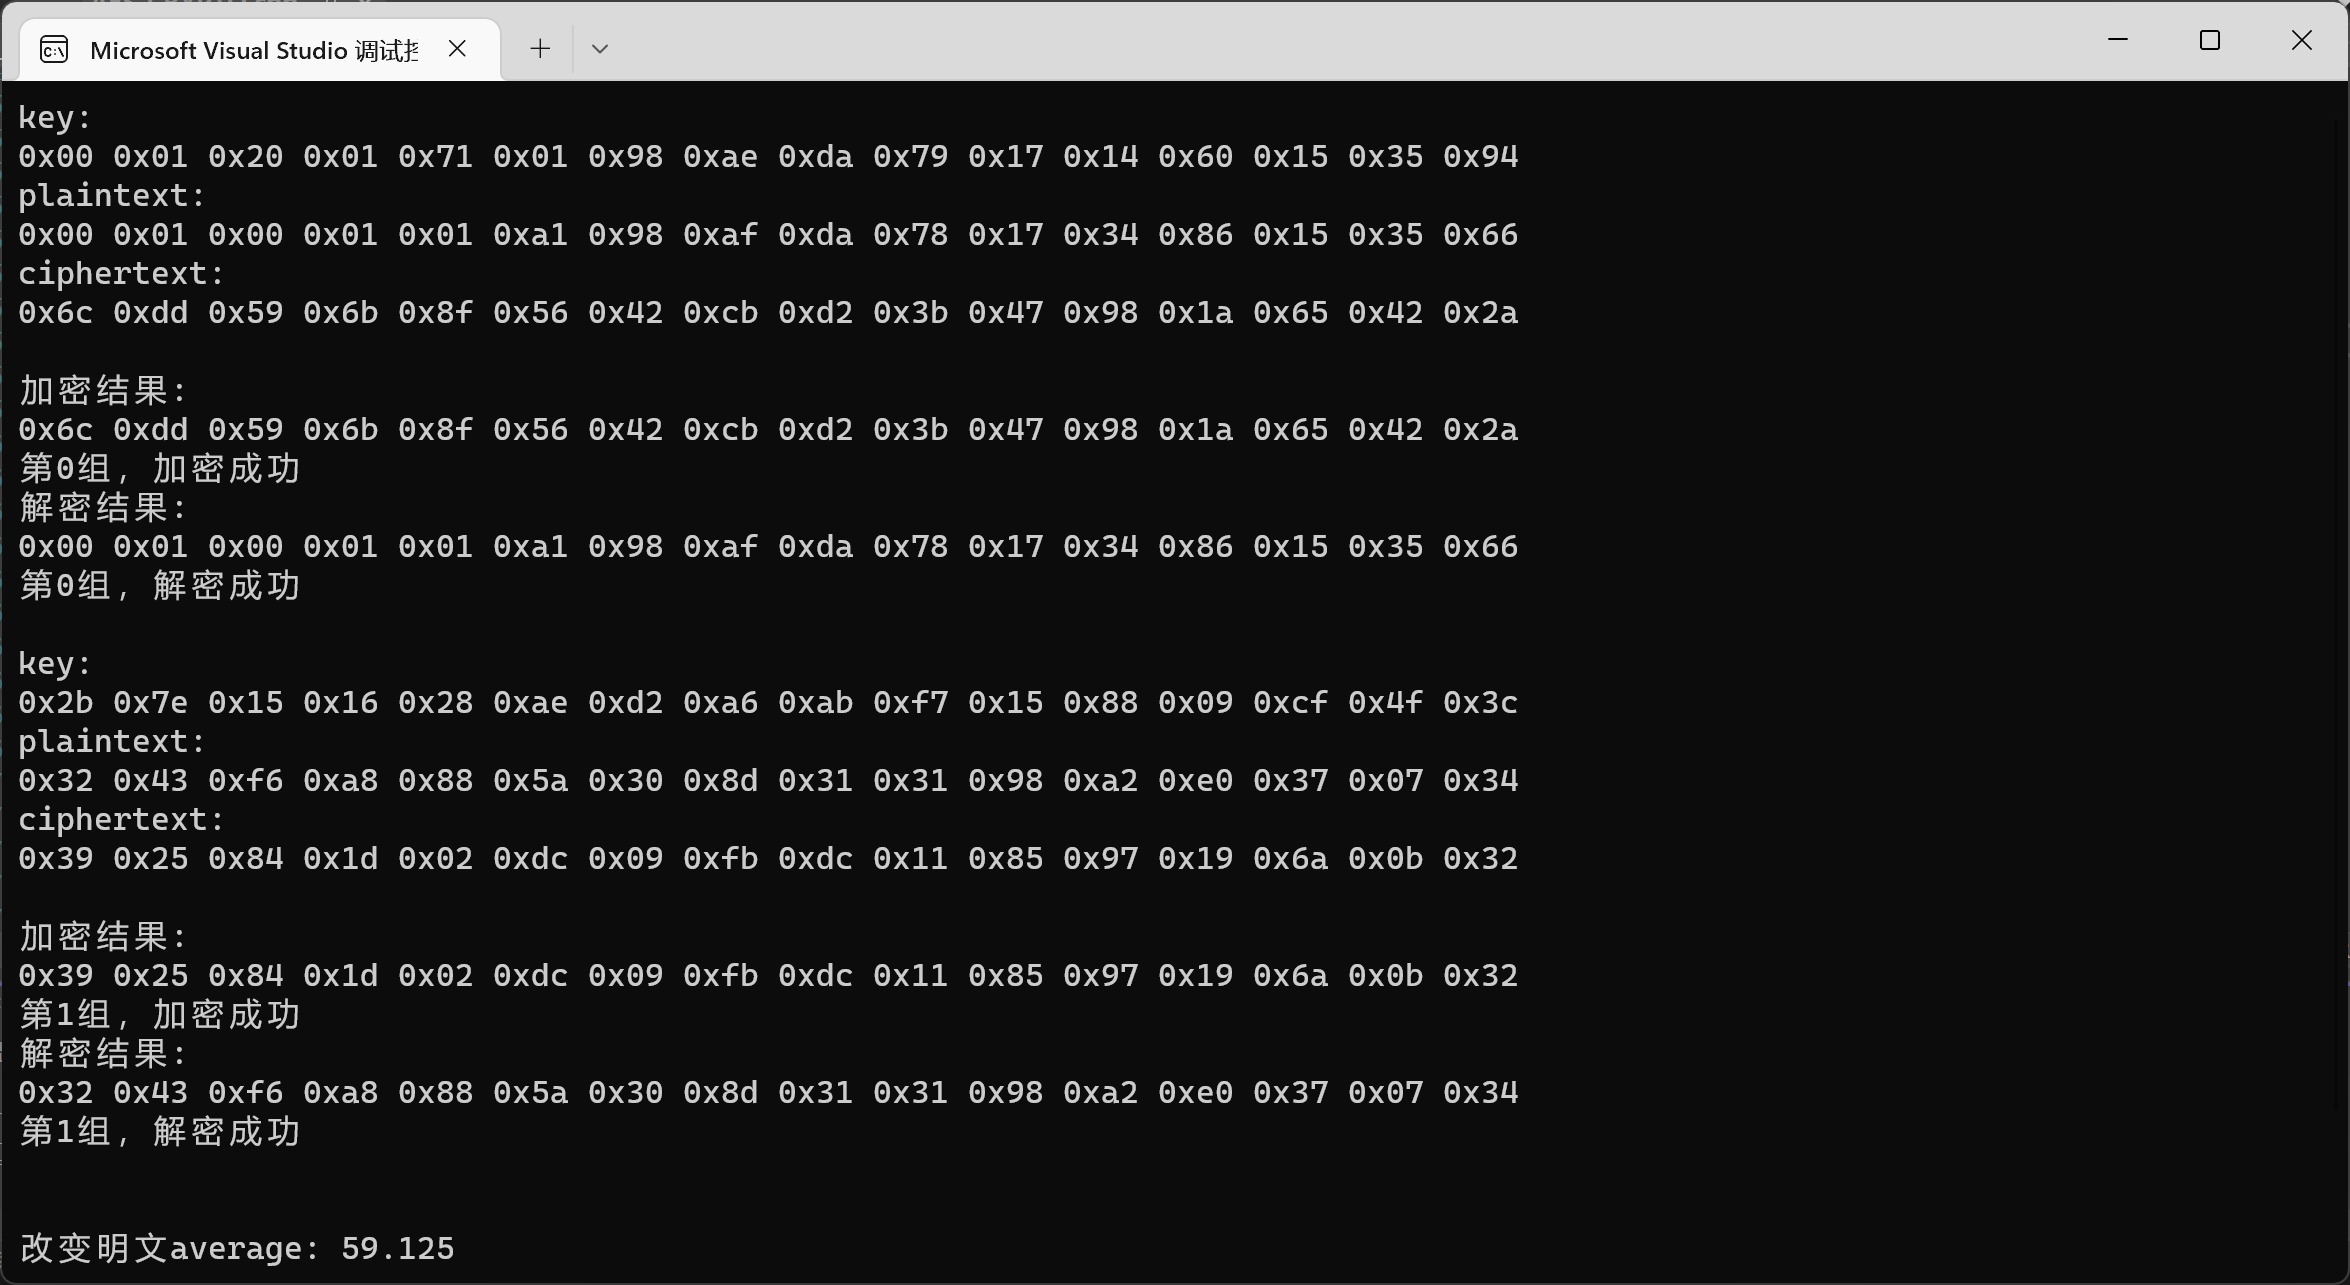
\includegraphics[height=10 CM]{figure/003}
	\caption{样例加解密结果}
	\label{fig:样例加解密结果}
\end{figure}
\begin{lstlisting}[language=c++]
S,rS,rC和测试样例见data.h
#include "data.h"
using namespace std;
string int2binstr(int text[4][4]) {
	string result;
	for (int i = 0; i < 4; i++) {
		for (int j = 0; j < 4; j++) {
			string str = "00000000";
			int temp = text[j][i];
			for (int k = 7; k >= 0; k--) {
				str[k] = '0' + temp % 2;
				temp /= 2;
			}
			result += str;
		}
	}
	return result;
}
void binstr2int(int text[4][4], string str) {
	unsigned char* output = new unsigned char[16];
	for (int i = 0; i <= 15; i++) {
		int start = i * 8;
		int temp = 0;
		for (int j = start; j <= start + 7; j++) {
			int each = 1;
			for (int s = 1; s <= 7 - j + start; s++) {
				each *= 2;
			}
			if (str[i] == '1') {
				temp += each;
			}
		}
		output[i] = temp;
	}
	for (int i = 0; i < 4; i++) {
		for (int j = 0; j < 4; j++) {
			text[j][i] = output[j * 4 + i];
		}
	}
}
//基本运算
int mult(int a, int b)
{
	int third = b & 0x8;//b>=8
	int second = b & 0x4;
	int first = b & 0x2;
	int firstMod = b % 2;
	int res = 0;
	if (third)
	{
		int temp = a;
		for (int i = 1; i <= 3; ++i)
		{
			temp = temp << 1;
			if (temp >= 256)
			{
				temp = temp ^ 0x11b;
			}
		}
		temp = temp % 256;
		res = res ^ temp;
	}
	if (second)
	{
		int temp = a;
		for (int i = 1; i <= 2; ++i)
		{
			temp = temp << 1;
			if (temp >= 256)
			{
				temp = temp ^ 0x11b;
			}
		}
		temp = temp % 256;
		res = res ^ temp;
	}
	if (first)
	{
		int temp = a;
		temp = temp << 1;
		if (temp >= 256)
		{
			temp = temp ^ 0x11b;
		}
		temp = temp % 256;
		res = res ^ temp;
	}
	if (firstMod)
	{
		res = res ^ a;
	}
	return res;
}
void KeyExpansion(int key[4][4], int Exp[11][4][4])//密钥拓展
{
	for (int i = 0; i < 4; ++i)
	{
		for (int j = 0; j < 4; j++)
		{
			Exp[0][i][j] = key[j][i];
		}
	}
	for (int i = 1; i < 11; ++i)
	{
		for (int j = 0; j < 4; ++j)
		{
			int temp[4];
			if (j == 0)
			{
				temp[0] = Exp[i - 1][3][1];
				temp[1] = Exp[i - 1][3][2];
				temp[2] = Exp[i - 1][3][3];
				temp[3] = Exp[i - 1][3][0];
				for (int k = 0; k < 4; ++k)
				{
					int m = temp[k];
					int row = m / 16;
					int col = m % 16;
					temp[k] = S[row][col];
					if (k == 0)
					{
						temp[k] = temp[k] ^ rC[i - 1];
					}
				}
			}
			else
			{
				temp[0] = Exp[i][j - 1][0];
				temp[1] = Exp[i][j - 1][1];
				temp[2] = Exp[i][j - 1][2];
				temp[3] = Exp[i][j - 1][3];
			}
			for (int x = 0; x < 4; x++)
			{
				Exp[i][j][x] = Exp[i - 1][j][x] ^ temp[x];
			}
		}
	}
}
void ByteSub(int input[4][4], int type)//字节变换
{
	for (int i = 0; i < 4; i++)
	{
		for (int j = 0; j < 4; j++)
		{
			int temp = input[i][j];
			int row = temp / 16;
			int col = temp % 16;
			if (type == 1)
			{
				input[i][j] = S[row][col];
			}
			if (type == 0)
			{
				input[i][j] = rS[row][col];
			}
		}
	}
}
void ShiftRow(int input[4][4], int type) //行移位变换
{
	for (int i = 0; i < 4; i++)
	{
		for (int j = 0; j < i; j++)
		{
			if (type == 1)
			{
				int temp = input[i][0];
				input[i][0] = input[i][1];
				input[i][1] = input[i][2];
				input[i][2] = input[i][3];
				input[i][3] = temp;
			}
			else
			{
				int temp = input[i][3];
				input[i][3] = input[i][2];
				input[i][2] = input[i][1];
				input[i][1] = input[i][0];
				input[i][0] = temp;
			}
		}
	}
}
void MixColumn(int input[4][4], int type)//列混合变换
{
	for (int i = 0; i < 4; i++)
	{
		int t0 = input[0][i];
		int t1 = input[1][i];
		int t2 = input[2][i];
		int t3 = input[3][i];
		if (type == 1)
		{
			input[0][i] = mult(t0, 2) ^ mult(t1, 3) ^ t2 ^ t3;
			input[1][i] = t0 ^ mult(t1, 2) ^ mult(t2, 3) ^ t3;
			input[2][i] = t0 ^ t1 ^ mult(t2, 2) ^ mult(t3, 3);
			input[3][i] = mult(t0, 3) ^ t1 ^ t2 ^ mult(t3, 2);
		}
		else
		{
			input[0][i] = mult(t0, 14) ^ mult(t1, 11) ^ mult(t2, 13) ^ mult(t3, 9);
			input[1][i] = mult(t0, 9) ^ mult(t1, 14) ^ mult(t2, 11) ^ mult(t3, 13);
			input[2][i] = mult(t0, 13) ^ mult(t1, 9) ^ mult(t2, 14) ^ mult(t3, 11);
			input[3][i] = mult(t0, 11) ^ mult(t1, 13) ^ mult(t2, 9) ^ mult(t3, 14);
		}
	}
}
void AddRoundKey(int input[4][4], int key[4][4])//密钥加
{
	for (int i = 0; i < 4; ++i)
	{
		for (int j = 0; j < 4; j++)
		{
			input[i][j] = input[i][j] ^ key[j][i];
		}
	}
}
void Encrypt(int plaintext[4][4], int key[4][4])//加密
{
	int en_or_de = 1;
	int Exp[11][4][4];
	KeyExpansion(key, Exp);
	AddRoundKey(plaintext, Exp[0]);
	for (int i = 1; i <= 10; ++i)
	{
		ByteSub(plaintext, en_or_de);
		ShiftRow(plaintext, en_or_de);
		if (i != 10)
		{
			MixColumn(plaintext, en_or_de);
		}
		AddRoundKey(plaintext, Exp[i]);
	}
}
void Decrypt(int ciphertext[4][4], int key[4][4])//解密
{
	int en_or_de = 0;
	int Exp[11][4][4];
	KeyExpansion(key, Exp);
	AddRoundKey(ciphertext, Exp[10]);
	for (int i = 9; i >= 0; --i)
	{
		ShiftRow(ciphertext, en_or_de);
		ByteSub(ciphertext, en_or_de);
		AddRoundKey(ciphertext, Exp[i]);
		if (i != 0)
		{
			MixColumn(ciphertext, en_or_de);
		}		
	}
}
	
int main() {
	int key0[4][4], plaintext0[4][4], ciphertext0[4][4];//记录第一组数据,用于后续雪崩检验
	for (int k = 0; k < 2; k++)
	{
		int key[4][4], plaintext[4][4], ciphertext[4][4];
		//cout << "输入密文(hex 128bit):";
		for (int i = 0; i < 4; i++)
		{
			for (int j = 0; j < 4; j++)
			{
				plaintext[j][i] = cases[k].plaintext[i][j];
				ciphertext[j][i] = cases[k].ciphertext[i][j];
				key[j][i] = cases[k].key[i][j];
				
				plaintext0[j][i] = cases[0].plaintext[i][j];
				ciphertext0[j][i] = cases[0].ciphertext[i][j];
				key0[j][i] = cases[0].key[i][j];
			}
		}
		Encrypt(plaintext, key);//检查加密结果
		bool t = true;//判断加密结果与样例结果是否一致
		for (int i = 0; i < 4; i++)
		{
			for (int j = 0; j < 4; j++)
			{
				if (plaintext[j][i] != cases[k].ciphertext[i][j])
				{
					cout << "第" << k << "组,加密失败" << endl;
					t = false;
					break;
				}
			}
		}
		if (t)
		cout << "第" << k << "组,加密成功" << endl;
		Decrypt(ciphertext, key);//检查解密结果
		bool t1 = true;//判断解密结果是否与样例一致
		for (int i = 0; i < 4; i++)
		{
			for (int j = 0; j < 4; j++)
			{
				if (ciphertext[j][i] != cases[k].plaintext[i][j])
				{
					cout << "第" << k << "组,解密失败" << endl;
					t1 = false;
					break;
				}
			}
		}
		if (t1)
		cout << "第" << k << "组,解密成功" << endl << endl;
	}
	
	//雪崩效应检测
	int test_plaintext[4][4];
	int test_old[4][4];
	int test_key[4][4];
	for (int i = 0; i < 4; i++)
	{
		for (int j = 0; j < 4; j++)
		{
			test_plaintext[j][i] = cases[0].plaintext[i][j];
			test_old[j][i] = cases[0].plaintext[i][j];
			test_key[j][i] = cases[0].key[i][j];
		}
	}
	cout << endl;
		
	string result;
	cout << "改变明文" << endl;
	int num1 = 0;
	for (int i = 0; i <= 7; i++) {
		result = int2binstr(test_plaintext);
		if (result[i] == '0')
			result[i] = '1';
		else
			result[i] = '0';
		binstr2int(test_plaintext, result);
		Encrypt(test_plaintext, key0);
		int result_text = 0;
		string s_new = int2binstr(test_plaintext);
		string s = int2binstr(ciphertext0);
		for (int i = 0; i < 128; i++) {
			if (s_new[i] != s[i]) {
				result_text++;
			}
		}
		cout << "change plaintext[" << i << "]: " << result_text << endl;
		num1 += result_text;
	}
	cout << "average: " << (float)num1 / 8 << endl << endl;
	cout << "改变密钥" << endl;
	int num2 = 0;
	for (int i = 0; i <= 7; i++) {
		result = int2binstr(test_key);
		if (result[i] == '0')
			result[i] = '1';
		else
			result[i] = '0';
		binstr2int(test_key, result);
		Encrypt(test_old, test_key);
		int result_text = 0;
		string s_new = int2binstr(test_old);
		string s = int2binstr(ciphertext0);
		for (int i = 0; i < 128; i++) {
			if (s_new[i] != s[i]) {
				result_text++;
			}
		}
		cout << "change key[" << i << "]: " << result_text << endl;
		num2 += result_text;
	}
	cout << "average: " << (float)num2 / 8 << endl;
	return 0;
}
	
\end{lstlisting}
%\begin{enumerate}
%	\item \textbf {预处理器:}处理源代码中以\#开始的预编译指令,例如展开所有宏定义、插入\#include指向的文件等,以获得经过预处理的源程序。
%	
%	\item \textbf {编译器:}将预处理器处理过的源程序文件翻译成为标准的汇编语言以供计算机阅读。
%	
%	\item \textbf {汇编器:}将汇编语言指令翻译成机器语言指令,并将汇编语言程序打包成可重定位目标程序。
%	
%	\item \textbf {链接器:}将可重定位的机器代码和相应的一些目标文件以及库文件连接在一起,形成真正能在机器上运行的目标机器代码。
%\end{enumerate}

%\begin{figure}[thbp!]
%	\centering
%	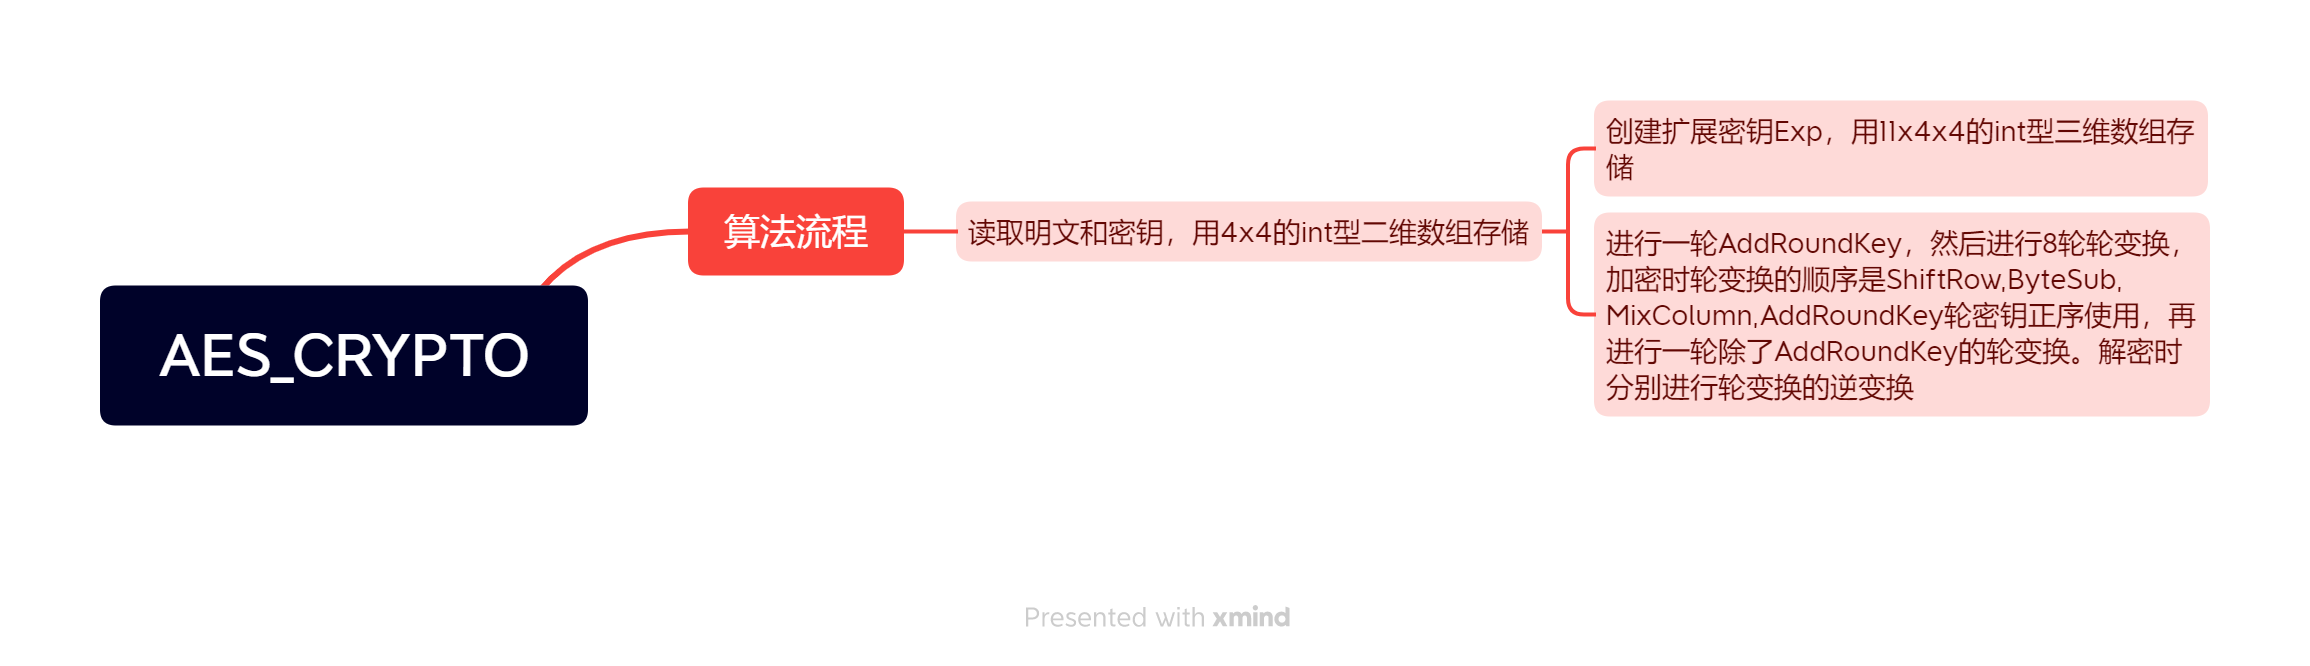
\includegraphics[height=6.8 CM]{figure/001}
%	\caption{语言处理过程图示}
%	\label{fig:语言处理过程图示}
%\end{figure}

























